\documentclass[]{article}

\usepackage{graphicx}

%opening
\title{}
\author{}

\begin{document}

\maketitle

\section{Solver parallelization}

\subsection{Simulation grid partitioning}

\paragraph{Slab decomposition}

\paragraph{Pencil decomposition}

\paragraph{Performance comparison}
Figure \ref{fig:strongscaling} illustrates the performance of aforementioned grid partitioning strategies, based on benchmark results of a strong scaling test. The test is performed on the state-of-the-art 2016 Flemish Tier1 supercomputer BrENIAC, equipped with compute nodes containing two Intel Xeon E5-2680v4 processors (2.4GHz, 14 cores per processor, Broadwell architecture) which are interconnected by a high-bandwidth and low-latency EDR Infiniband network. The scaling test is performed for a canonical high Reynolds number half-channel flow, using a simulation grid of $512 \times 256 \times 256 \approx 33.5 \times 10^6$ grid points. (PUT THIS INTO CONTEXT)


Figure \ref{fig:strongscaling}a shows the walltime per timestep as a function of the amount of processors, which is a measure for the absolute computational cost in terms of time-to-solution. ADD DISCUSSION HERE

Figure \ref{fig:strongscaling}b shows the parallel efficiency, defined as the ratio between the ideal walltime per timestep assuming perfect linear scalability from the reference case on the one hand, and the actual walltime per timestep for a given amount of cores on the other. In contrast to the walltime shown in Figure \ref{fig:strongscaling}a, the parallel efficiency in Figure \ref{fig:strongscaling}b is a measure for computational cost in terms of CPU-hours. It can be seen that for simulations on a small amount of processor cores the benefit of eliminating the $\verb|MPI_COMM_Y|$ communicator by having a single centralized $\verb|MPI_COMM_X|$ all-to-all communication outweighs the detrimental effects of having a larger $\verb|MPI_COMM_X|$ communicator. However, as the number of processor cores increases, the larger all-to-all causes a significant drop in parallel efficiency for a slab decomposition. Pencil decompositions on the other hand allow to convert the single large all-to-all communication step into 3 smaller all-to-alls. Figure \ref{fig:strongscaling}b indicates that, by doing so, the sharp decline in parallel efficiency can be mitigated up until a much larger core count. 

\begin{figure}
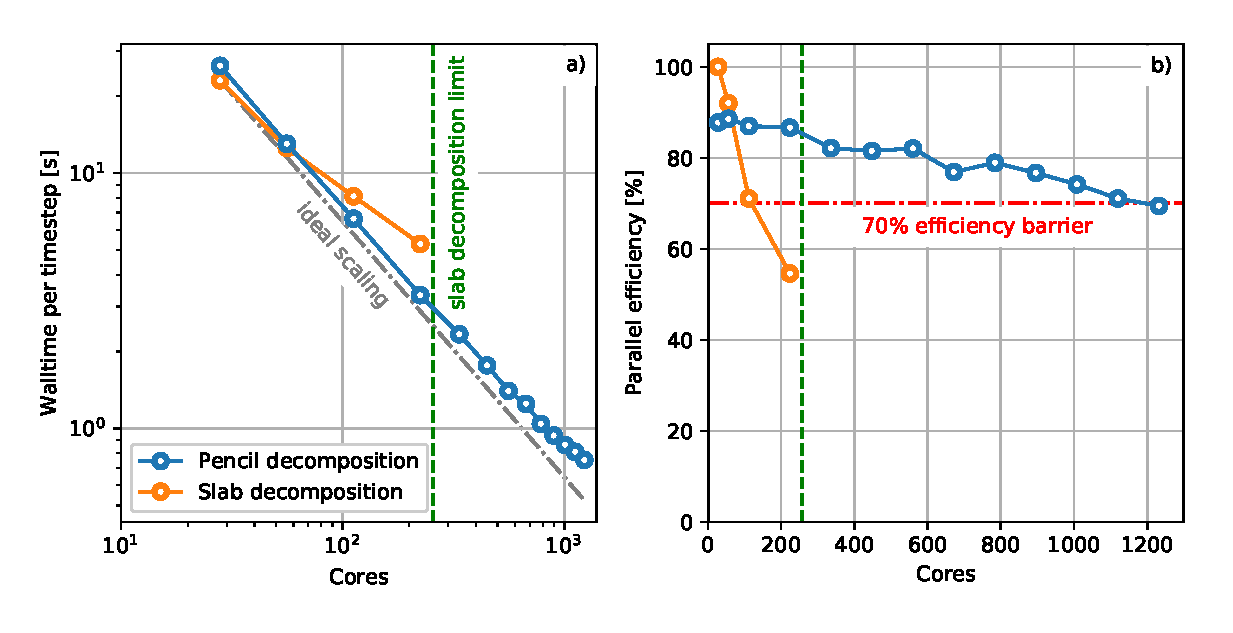
\includegraphics[width=\textwidth]{meth_strong_scaling.eps}
\caption{Strong scaling plot for SP-Wind solver. \emph{a)} Walltime per timestep within Runge-Kutta time integration. \emph{b)} Parallel efficiency in comparison to single-node slab partitioning. \label{fig:strongscaling}}
\end{figure}
\subsection{Processor mapping \& intranode communication}


\end{document}
